\section{Biokompatibilität}

\subsection{Kurzbeschreibung des Experiments}
Verschiedene Materialien werden auf ihre in-vitro-Zytotoxität hin untersucht.
Hierzu wird eine Hefelösung verwendet. Die zu untersuchenden Matierialien
sind in einem Glasbehälter mit der Hefelösung. Von dieser Hefelösung wird eine
Probe entnommen von 20$\mu$L welcher 20$\mu$L Methylenblau beigemischt wird.
Nach 15 Minuten Ruhezeit bei normalen Raumbedingungen werden die verschiedenen
Proben unter dem Mikroskop betrachtet. Dabei wird ausgeweret, wie viele
Hefezellen tot sind. Tote Zellen erhalten durch das Methylenblau eine blaue
Färbung.

\subsection{Ergebnisse}

\begin{figure}[h!]
	\centering
	\begin{subfigure}[b]{0.45\textwidth}
		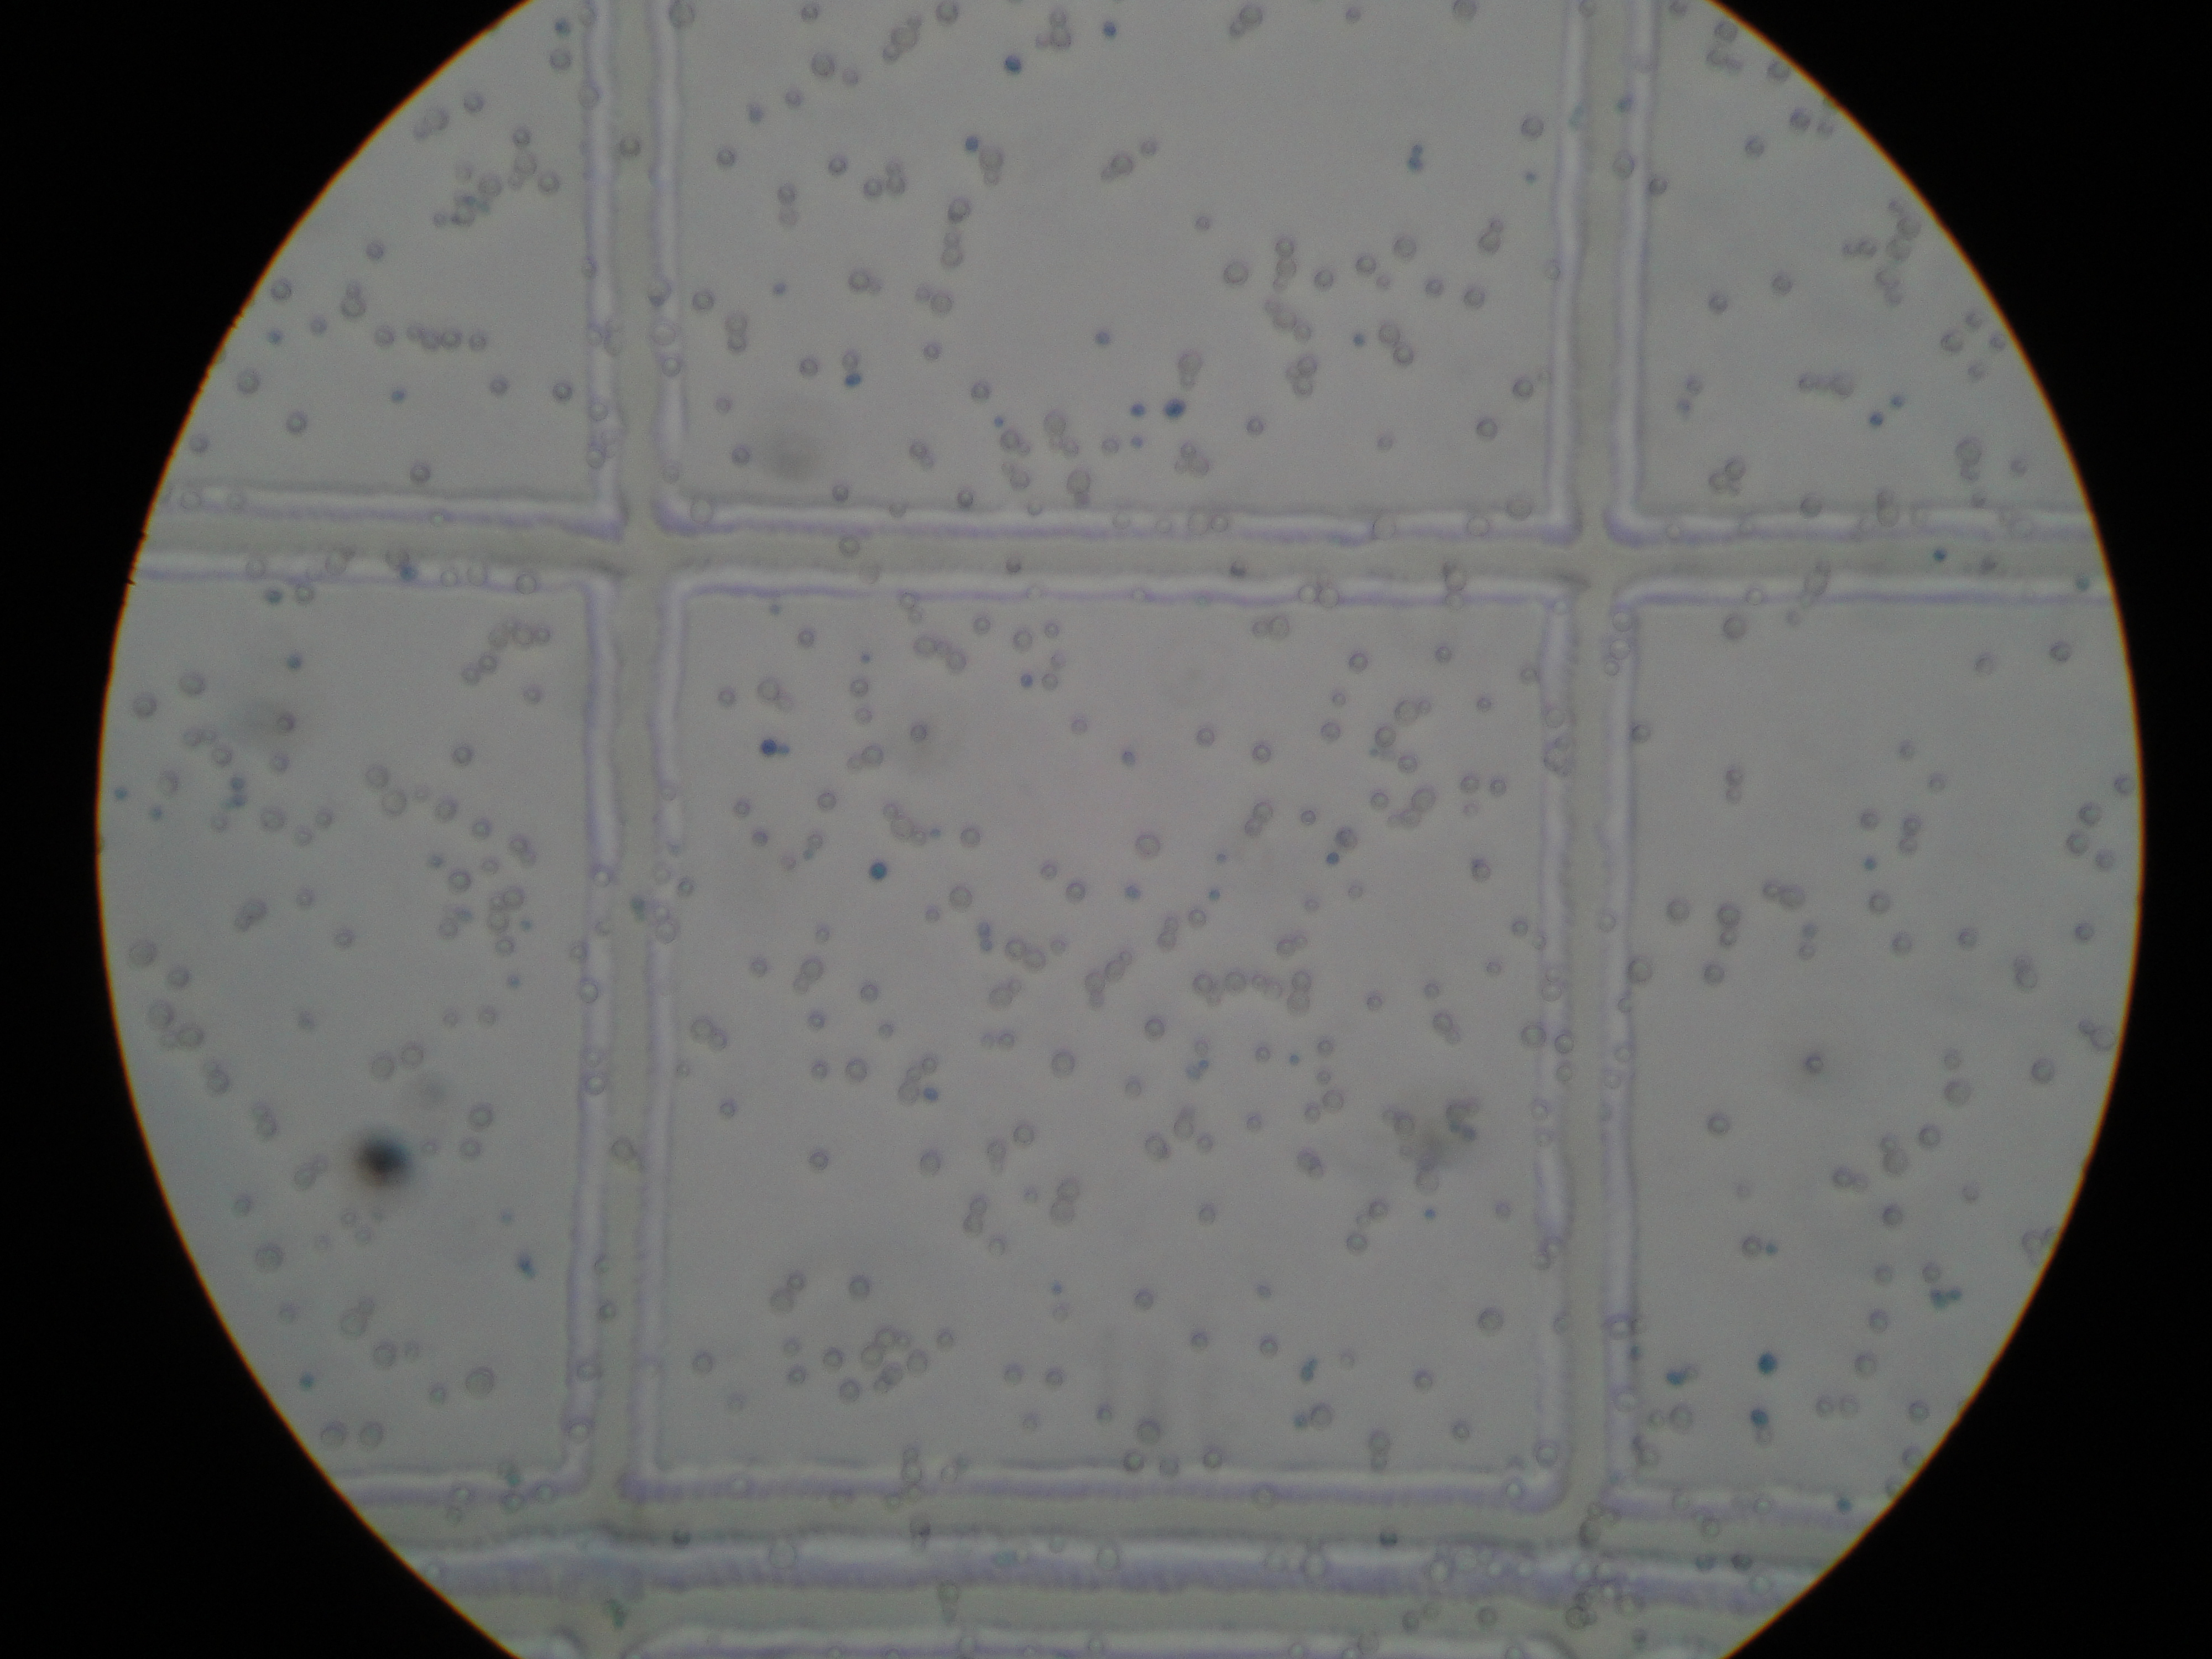
\includegraphics[width=1\textwidth]{../images/bio_01.jpg}
		\caption{Probe A - 12 tote Hefezellen}
	\end{subfigure}
	\begin{subfigure}[b]{0.45\textwidth}
		\includegraphics[width=1\textwidth]{../images/bio_04.jpg}
		\caption{Probe B - 45 tote Hefezellen}
	\end{subfigure}

	\begin{subfigure}[b]{0.45\textwidth}
		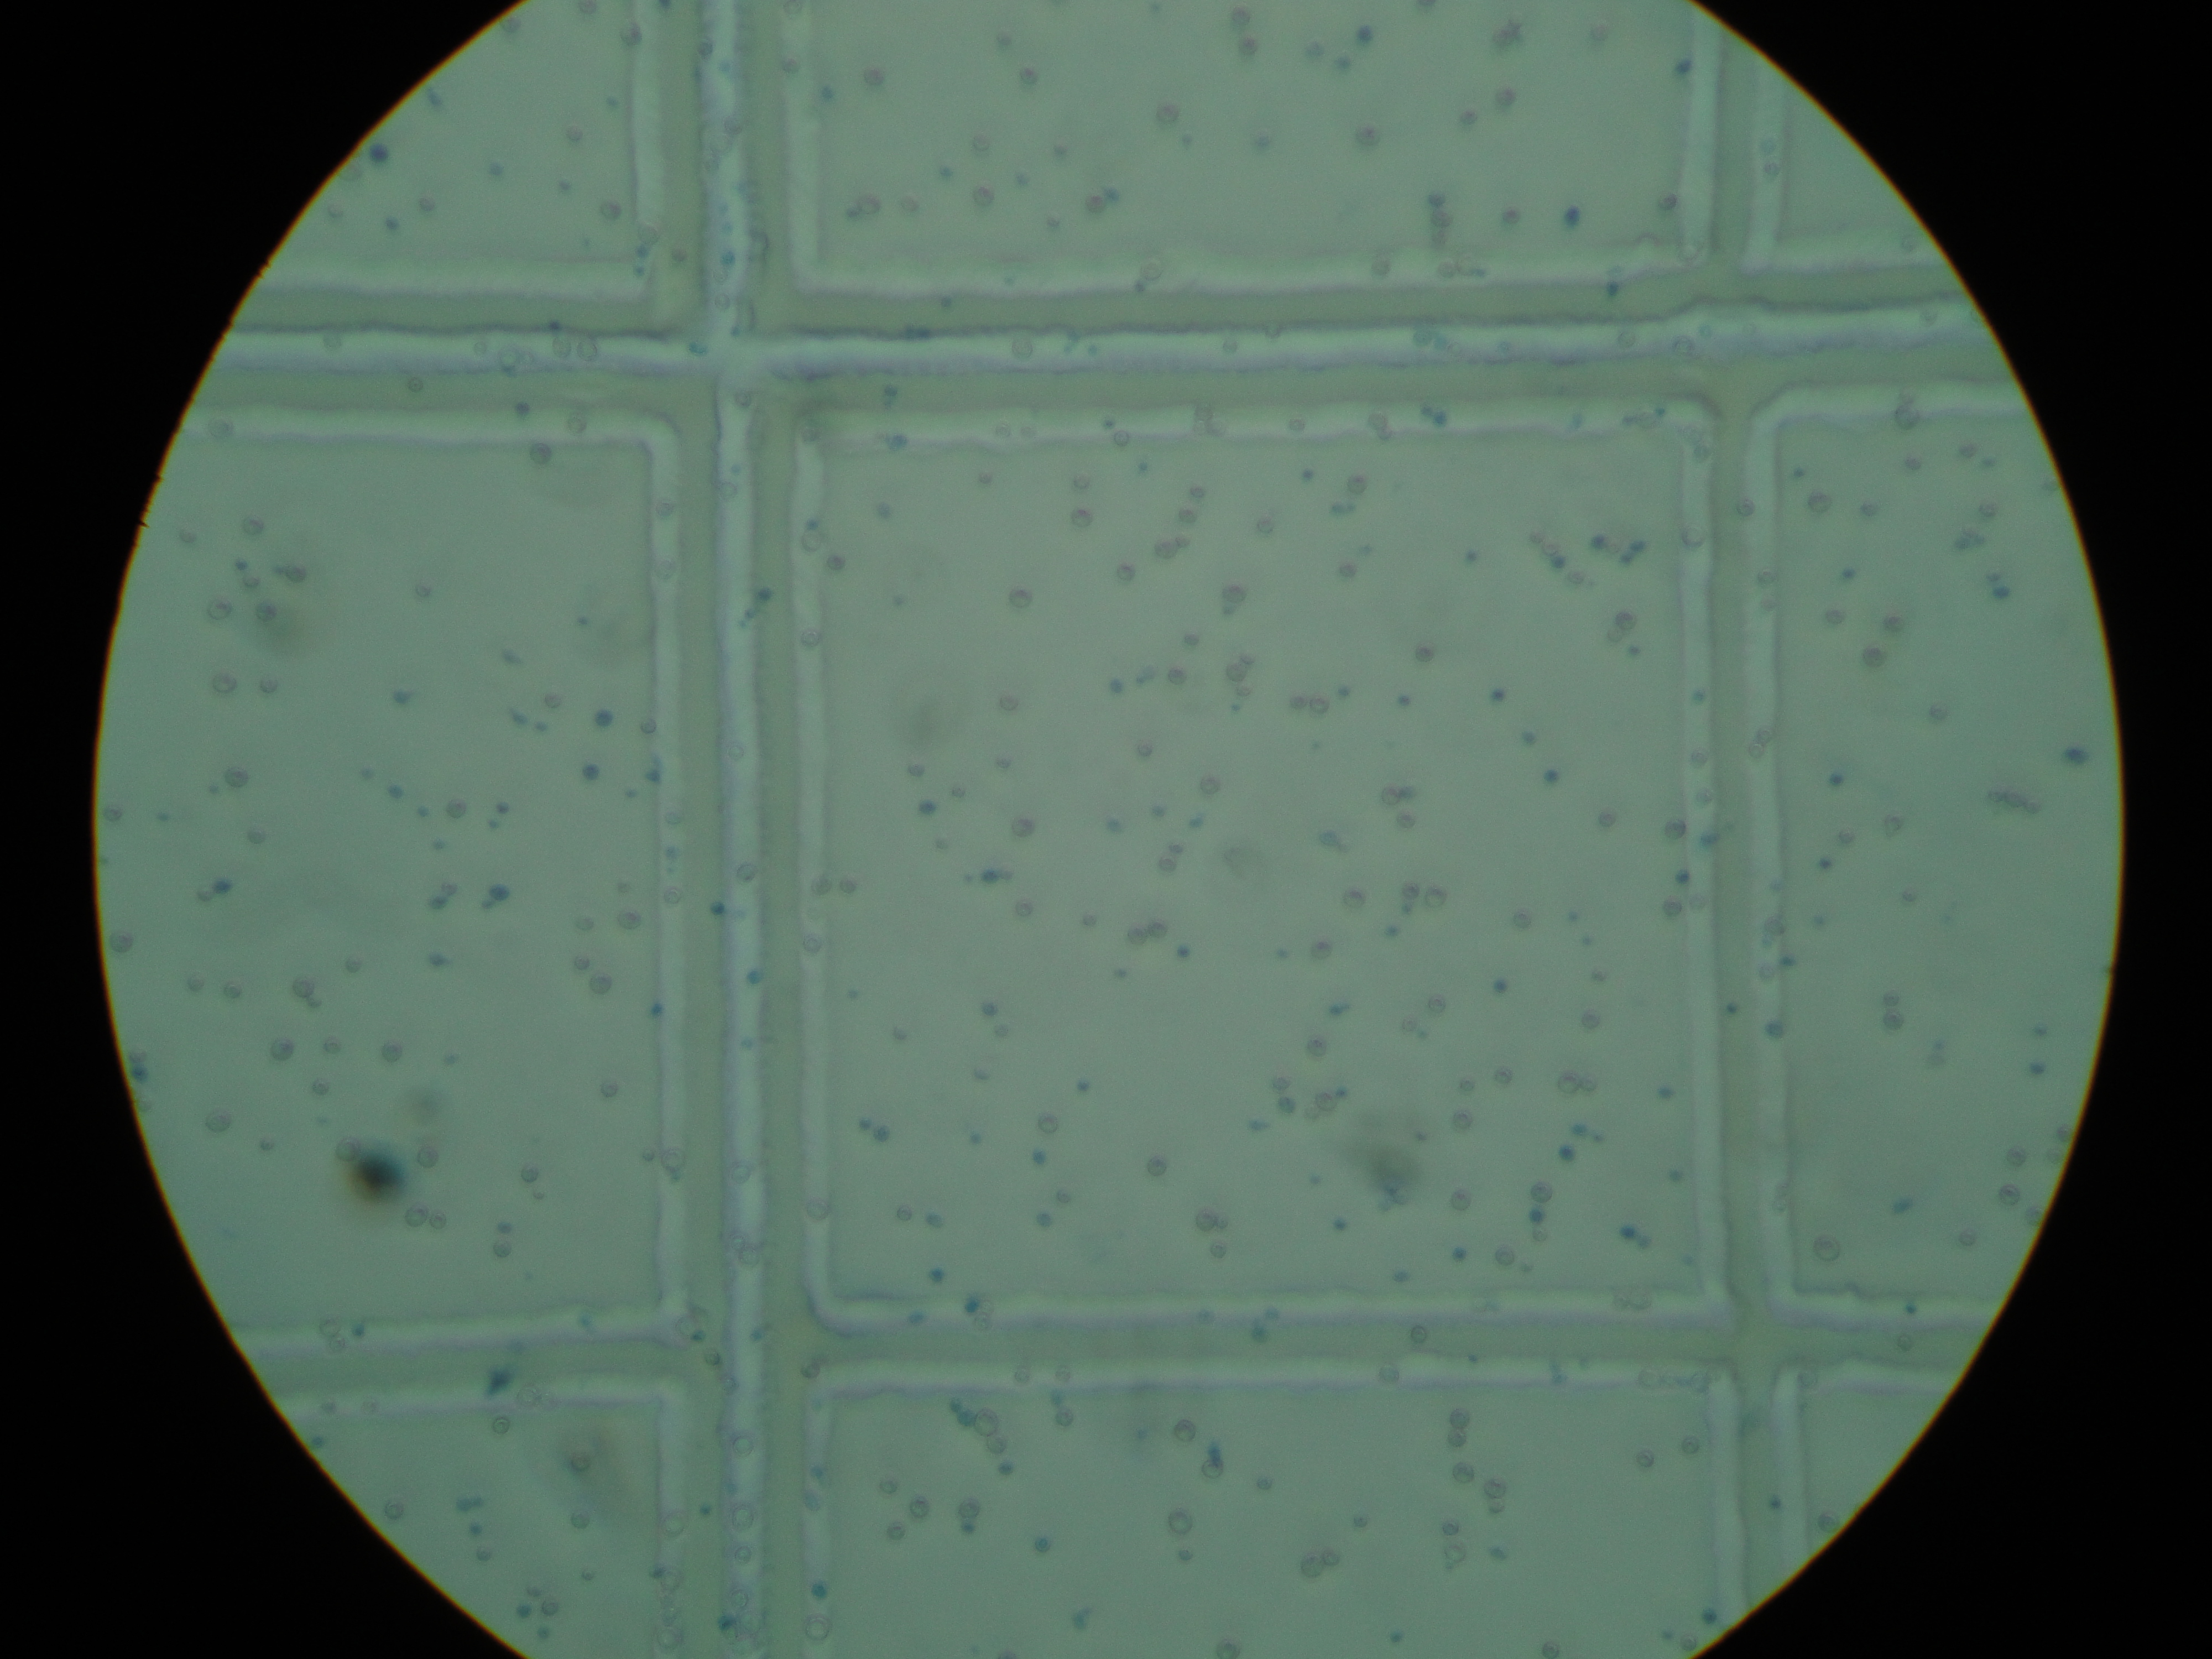
\includegraphics[width=1\textwidth]{../images/bio_05.jpg}
		\caption{Probe C - 60 tote Hefezellen}
	\end{subfigure}
	\begin{subfigure}[b]{0.45\textwidth}
		\includegraphics[width=1\textwidth]{../images/bio_06.jpg}
		\caption{Probe D - keine toten Hefezellen}
	\end{subfigure}

	\begin{subfigure}[b]{0.45\textwidth}
		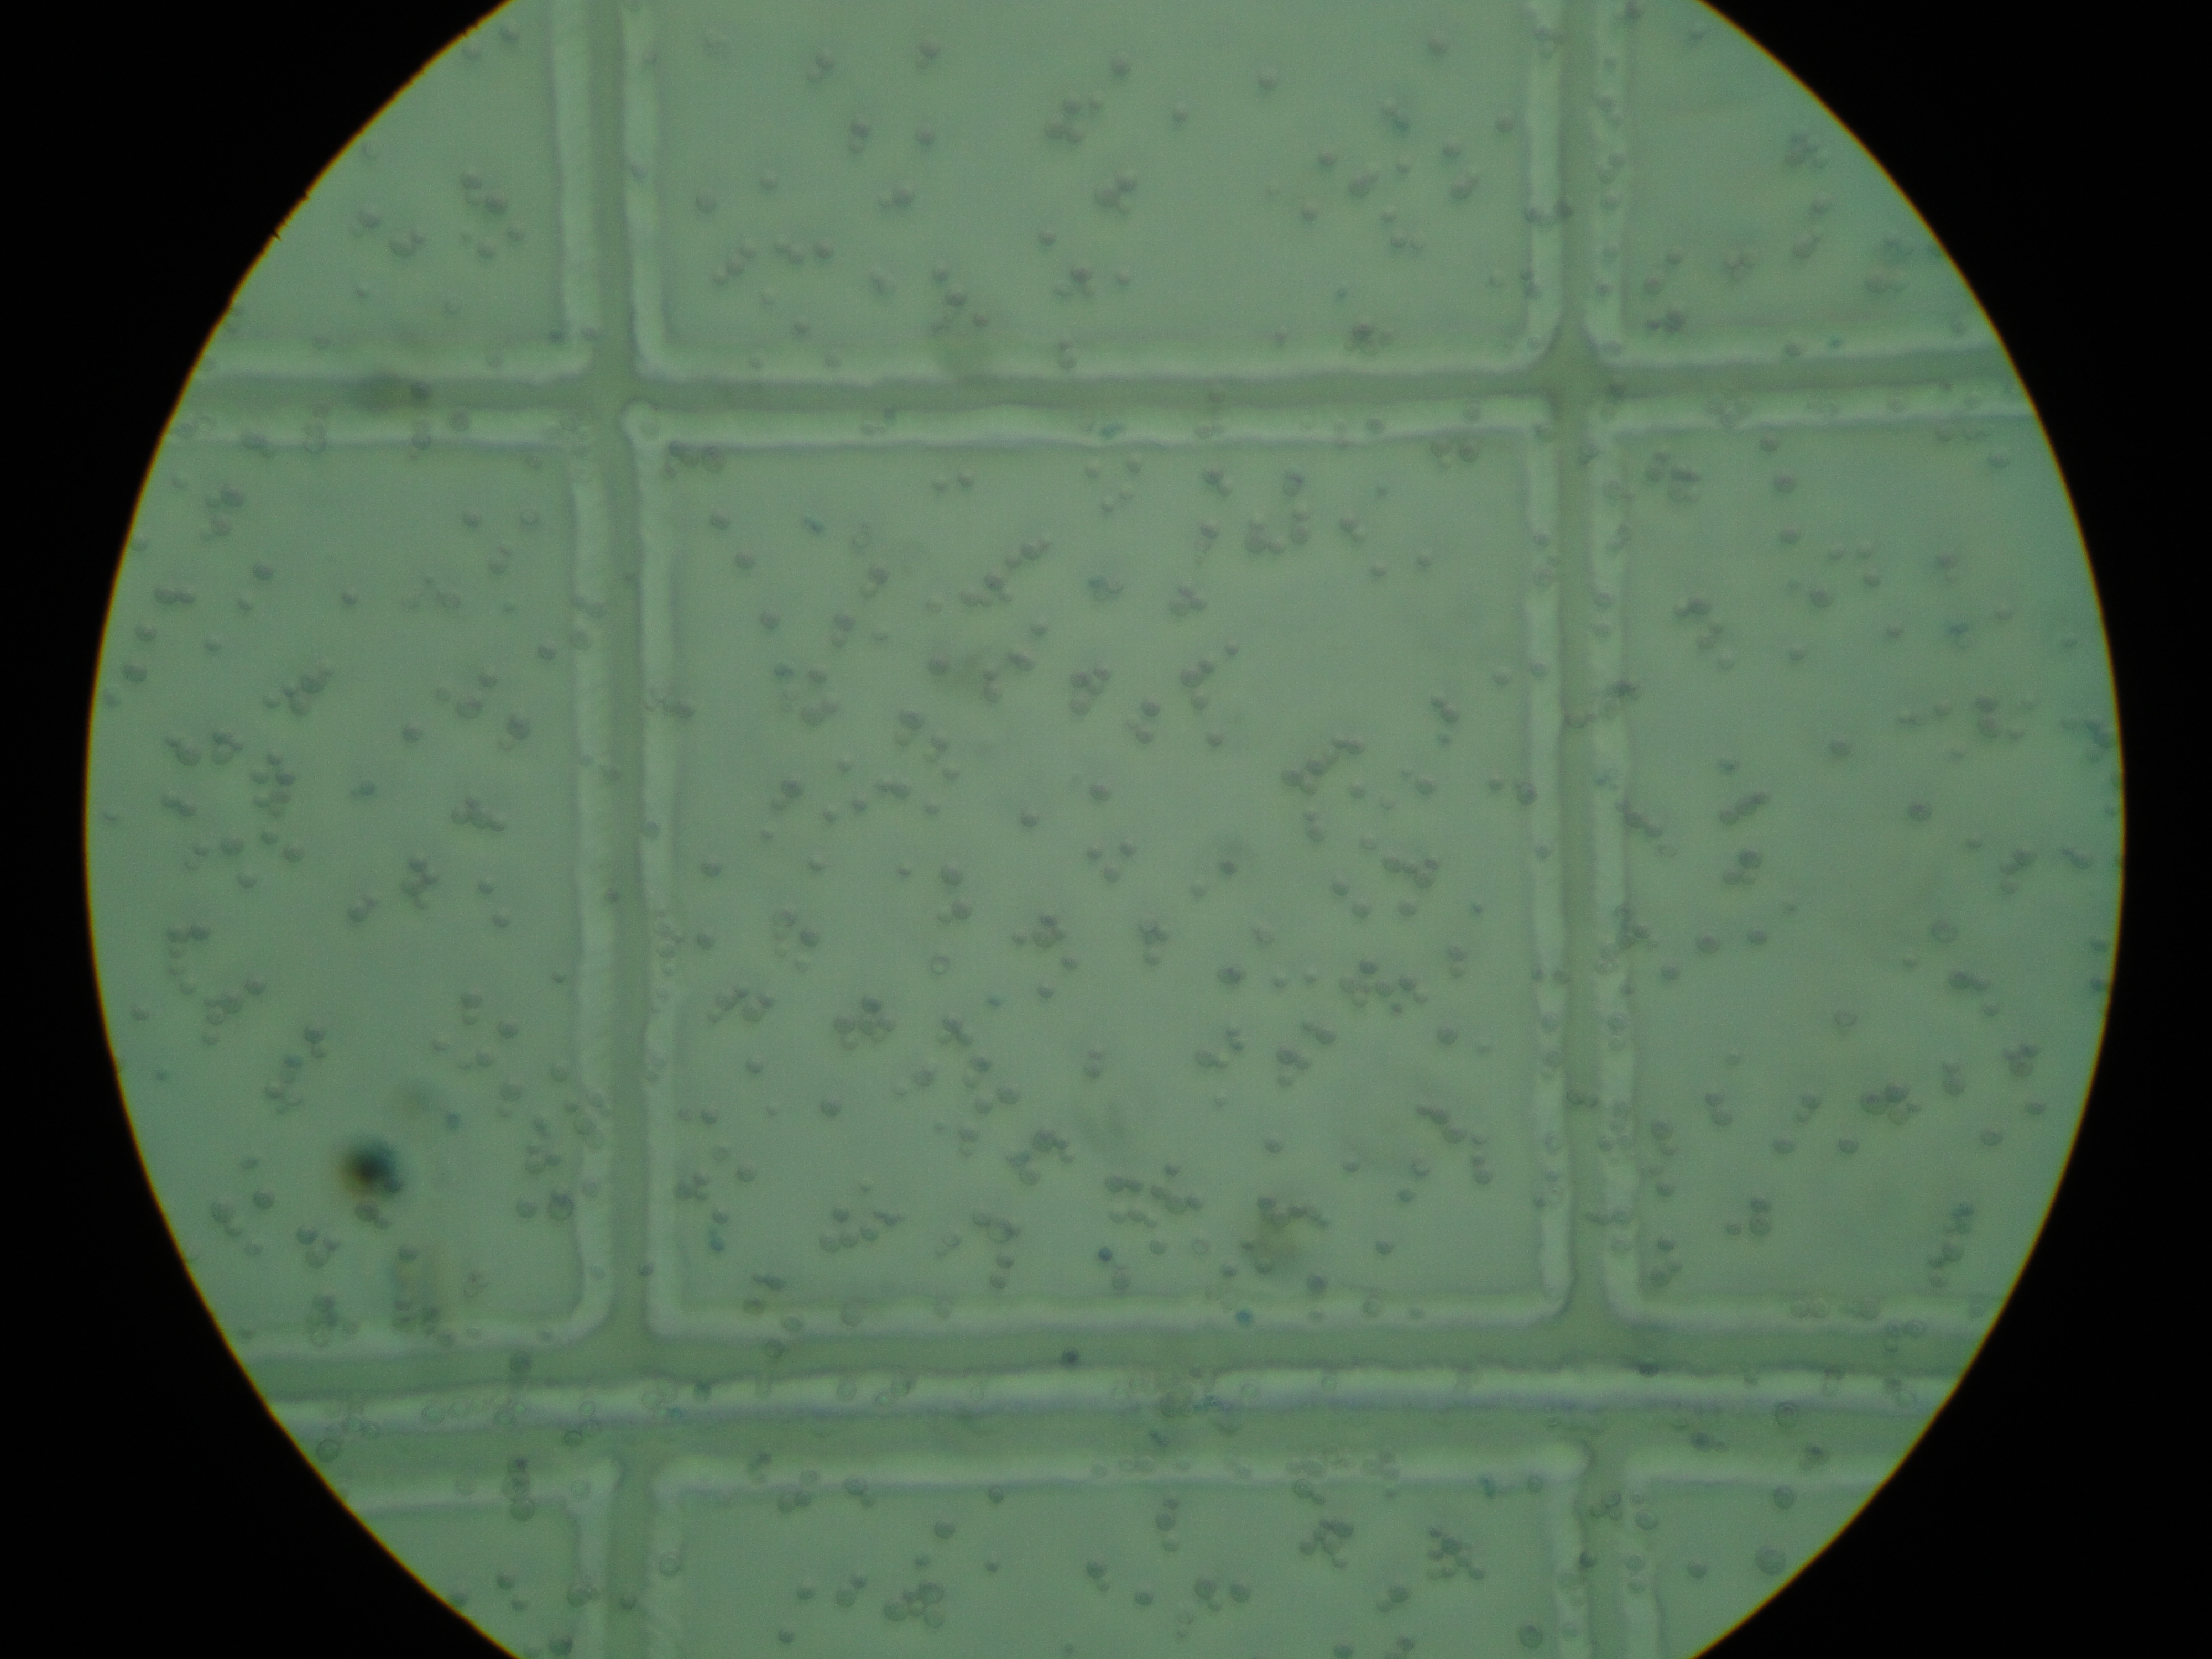
\includegraphics[width=1\textwidth]{../images/bio_07.jpg}
		\caption{Probe E - keine toten Hefezellen}
	\end{subfigure}
\end{figure}

\newpage
\clearpage
\subsection{Fazit}
